\documentclass[12pt,a4paper,oneside,article]{memoir}

% LAYOUT
\setulmarginsandblock{0.7\uppermargin}{0.8\lowermargin}{*}
\usepackage{mylayout}


% LANGUAGE AND FONT
\setmainlanguage{english}
\setmainfont[Ligatures={TeX},Mapping={tex-text},Numbers={OldStyle}]{Linux Libertine O}
\setmonofont[Scale=0.8]{DejaVu Sans Mono}

% PDF SETUP
\usepackage[unicode,bookmarks, colorlinks, breaklinks,
pdftitle={S-114.4202: Exercise report},
pdfauthor={Ville Väänänen},
pdfproducer={xetex}
]{hyperref}
\hypersetup{linkcolor=black,citecolor=black,filecolor=black,urlcolor=MidnightBlue} 

\usepackage[shadow]{todonotes}

% MATH
\usepackage{mymath}
\everymath{\displaystyle}

\usepackage{listings}
\lstset{ %
	language=R,                % choose the language of the code
	basicstyle=\footnotesize\ttfamily,% the size of the fonts that are used for the code 
	numbers=none,                   % where to put the line-numbers
	numberstyle=\footnotesize\ttfamily,      % the size of the fonts that are usedfor the line-numbers 
	stepnumber=5,                   % the step between two line-numbers. If it's 1 each line 
	aboveskip=2\medskipamount,
	belowskip=2\medskipamount,                                % will be numbered
	numbersep=-5pt,                  % how far the line-numbers are from the code
	backgroundcolor=\color{white},  % choose the background color. You must add \usepackage{color}
	showspaces=false,               % show spaces adding particular underscores
	showstringspaces=false,         % underline spaces within strings
	showtabs=false,                 % show tabs within strings adding particular underscores
	frame=l,
	framesep=0pt,
	framexleftmargin=2mm,
	rulecolor=\color{light-gray},	                % adds a frame around the code
	tabsize=2,	                % sets default tabsize to 2 spaces
	caption=,
	captionpos=t,                   % sets the caption-position to bottom
	breaklines=true,                % sets automatic line breaking
	breakatwhitespace=false,        % sets if automatic breaks should only happen at whitespace
	emptylines=*1,
	keywordstyle=\color[rgb]{0,0,1},          % keywords in blue
    commentstyle=\color[gray]{.5}\itshape,               % comments
    stringstyle=\color[rgb]{.627,.126,.941},   % strings in purple
	%title=\lstname,                 % show the filename of files included with
	                                % also try caption instead of title
	escapeinside={\%*}{*)},         % if you want to add a comment within your code
            % if you want to add more keywords to the set
}

\newcommand{\Th}{\gv{\theta}}
\newcommand{\LH}{\Pdf{\v{Y}}{\Th}}
\newcommand{\LHf}[1]{\Pdf{\v{Y}}{#1}}
\newcommand{\LHh}{\Pdf{\v{Y}}{\hat{\Th}}}
\newcommand{\lLH}{L\!\left(\Th\right)}
\newcommand{\cLH}{\Pdf{\v{X},\v{Y}}{\Th}}
\newcommand{\lcLH}{\log\cLH}
\newcommand{\LB}{\mathcal{L}}
\newcommand{\Lb}{\mathfrak{L}}
\newcommand{\KL}[2]{\mathrm{KL}\left(#1\|#2\right)}


\newcommand{\course}{S-114.4202}
\newcommand{\coursename}{Special Course in Computational Engineering II}
\newcommand{\duedate}{\today}
\newcommand{\studentid}{63527M}
\renewcommand{\title}{Bear observations in Finland in 2010}
\author{Ville Väänänen}

% SECTION NUMBERING
%\setsecnumdepth{subsubsection}
\counterwithout{section}{chapter}
%\renewcommand{\thesubsubsection}{\thesubsection{\large\scshape\alph{subsubsection}}}
%\titleformat{\subsubsection}{\large\scshape}{\alph{subsubsection} )}{10pt}{}
%\titleformat{\section}{\Huge}{\thesection}{10pt}{}
%\titleformat{\subsection}{\Large}{\thesubsection}{10pt}{}


% BIBLIOGRAPHY
\usepackage[hyperref=true,  backend=biber]{biblatex} % TEXLIPSE BUG: backend cannot be first
\addbibresource{/Users/dennari/Documents/Bibtex/Bear_data.bib}

\checkandfixthelayout

\begin{document}



\mytitlepage

\section{Data description}

The bear observations in the year 2010 are plotted in figure~\ref{fig:bear}
and the population density of the municipalities (the number of people
in the municipality per its land area) is plotted in figure~\ref{fig:pdens}. 
As can be seen, there is some clustering which has to be associated with increased
probability of reporting due population density. Thus an interesting problem is,
how should we take into account the probability for an animal to get observed
in a given area? Is it directly proportional to population density? Is there some
other factors associated such as the amount of hunters in the area?

\begin{figure}[htbp]
  \begin{adjustwidth}{-2in}{-2in}
	  \centering
	  \subfloat[Bear observations in 2010]{\label{fig:bear}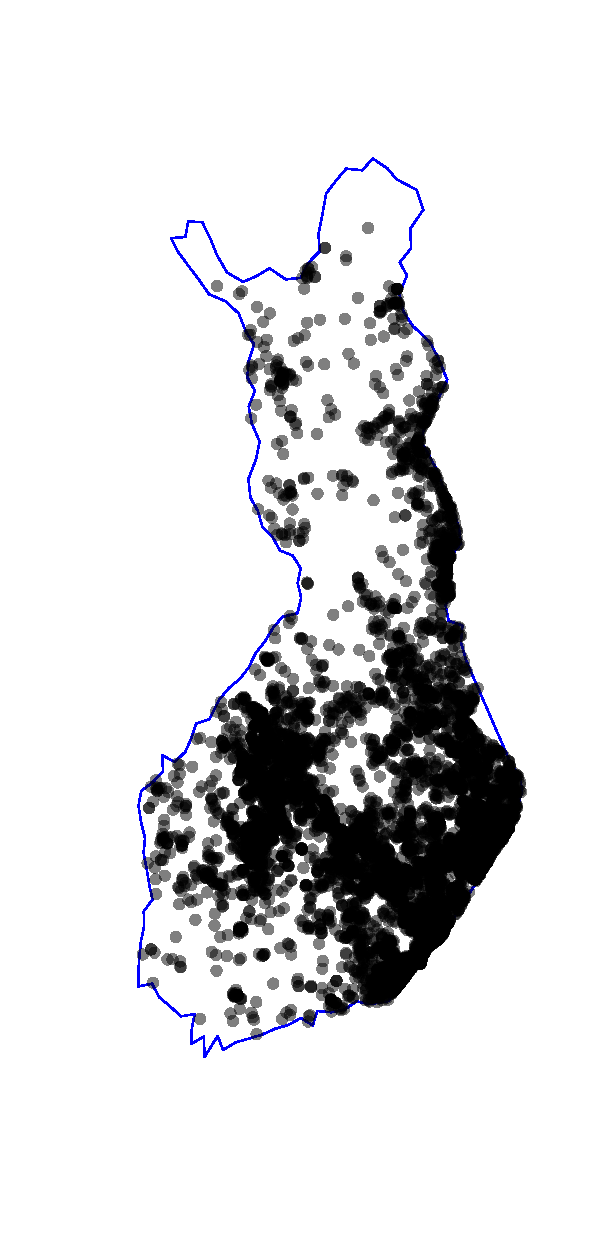
\includegraphics[width=0.6\textwidth]{b2010}}
	  \subfloat[Population density]{\label{fig:pdens}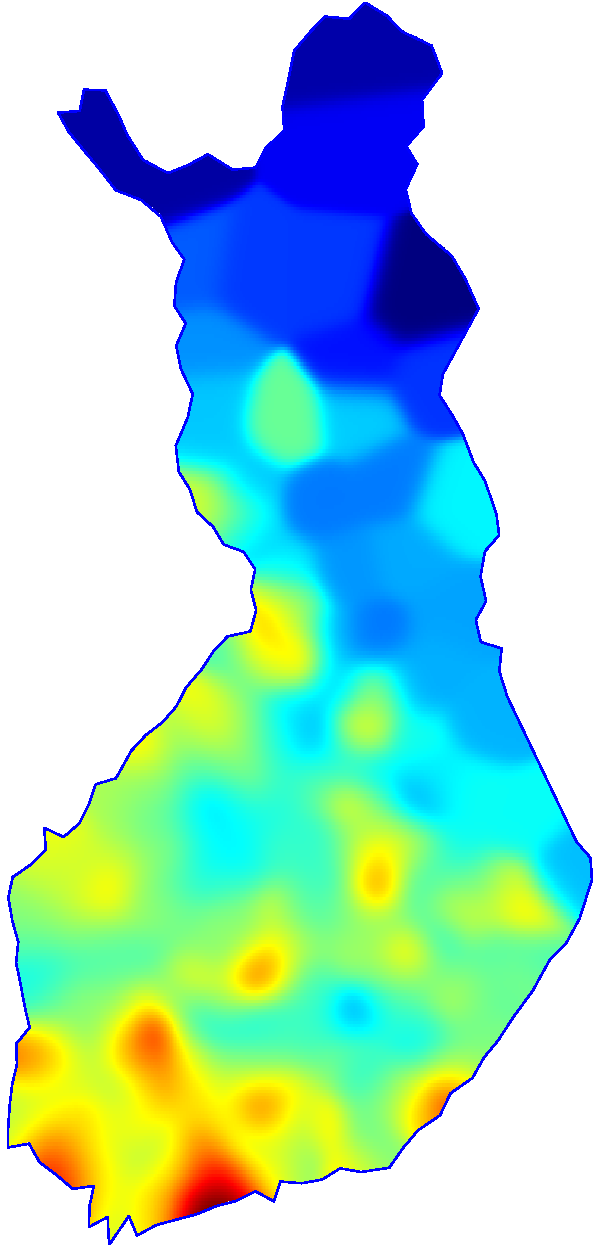
\includegraphics[width=0.6\textwidth]{pdens}}
  \end{adjustwidth}
  \caption{Bear observations in 2010 and the population density of Finland}
  \label{fig:bw2010}
\end{figure}


\section{Methods}


\subsection{Poisson process}

Poisson processes are considered the \emph{null} model in spatial 
point process statistics, since they exhibit \emph{complete spatial randomness} (CSR).
This means, that given the intensity field $\lambda(\v{s})$, the points of the process 
in two disjoint areas are indepedent.

Throughout the report, we will denote  vectors and vector valued functions with bold lower-case symbols and matrices
with bold upper case symbols. We will denote a \emph{spatial point process}, defined in some bounded region
$\Omega\subset\R^2$, with $\mathcal{X}$. A spatial point process can be considered a 
\emph{random finite subset} of, in this case, $\Omega$ \cite{Moller2007}. It is usually observed
in some bounded observation window $W\subset\Omega$.
A realisation of a point process is called a \emph{point pattern}
\begin{align}
	\mathcal{X}_W=\left\{\v{x}_1,\dots,\v{x}_n\right\},
	\label{eq:point_pattern}
\end{align}
where the points $\v{x}_k\in W$. 
The distribution of $\mathcal{X}$ can be defined by specifying the distribution of
the number of points $N(\Omega)$ (which we will also denote $N(\mathcal{X})$) and then the joint distribution of the $n$
points given $N(\Omega)=n$. Equivalently one can specify the distribution of $N(D)$, that is
is the number of points of $\mathcal{X}$ in any subset $D\subset \Omega$.

For the Poisson process we have
\begin{align}
	\PPdf{N(D)=k}{\lambda}=\frac{\Lambda(D)^k}{k!}e^{-\Lambda(D)},
	\label{eq:poisson}
\end{align}
where $\Lambda(D)=\defint{D}{}{\lambda(\v{s})}{\v{s}}$. Then, given the number of points,
the points are i.i.d so that the density is proportional to the intensity function. The joint distribution
of the number of points and the points, i.e. the likelihood, is then given by
\begin{align}
	\PPdf{\mathcal{X}}{\lambda}&=\PPdf{N(\mathcal{X})=n}{\lambda}\prod_{i=1}^n\frac{\lambda(\v{x}_i)}{\Lambda(\Omega)}
	\nonumber\\
	&=\frac{\Lambda(\Omega)^n}{n!}e^{-\Lambda(\Omega)}\prod_{i=1}^n\frac{\lambda(\v{x}_i)}{\Lambda(\Omega)} \nonumber\\
	&\propto \exp\left( -\defint{\Omega}{}{\lambda(\v{s})}{\v{s}} \right)\prod_{i=1}^n \lambda(\v{x}_i)
	\label{eq:poisson_lh}
\end{align}


\subsection{Cox processes}

Cox processes are a flexible family of point processes described by a 
\emph{random} intensity field. Thus they are also called doubly stochastic.
Given the random intensity field, a Cox process is a Poisson process.
In a log-Gaussian Cox process, the random latent intensity field has the form
\begin{align}
	\lambda(\v{s})&=e^{Z(\v{s})},\;\v{s}\in\R^2
	\label{eq:lambda_lgcp}
\end{align}
where $Z$ is a \emph{Gaussian random field} (also called a Gaussian process, $\mathcal{GP}$) defined by a 
mean function $\mu(\v{s})$ and a covariance function $c(\v{s},\v{s}')$ \cite{Moller2007}. 
In this report
a linear model will be used for the mean function, i.e
\begin{align}
	\mu(\v{s})&=\gv{\beta}^T\v{b}(\v{s}),
	\label{eq:lambda_mean}
\end{align}
where typically $b_1(\v{s})=1$, so that $\beta_1$ is the intercept. With this definition, possible
covariate data can be included directly in $\v{z}$. 

% The complete set of unknown parameters in our model
% is then
% \begin{align}
% 	\gv{\theta}&=\left[\gv{\theta}_Q^T,\;\gv{\beta}^T\right]^T
% 	\label{eq:parameters}
% \end{align}

\subsection{Latent Gaussian models}

Our aim is to be able to use a computationally efficient Bayesian procedure for inference
in latent Gaussian models called INLA (or integrated nested Laplace approximations) \cite{Rue2009}.
Latent Gaussian models are a large set of flexible models, where given a latent (unobserved) Gaussian 
random field the observations $\v{y}$ are independent and identically distributed with
an exponential family distribution \cite{Rue2009}. 
More precisely we have
\begin{align}
	Z(\v{s})|\gv{\theta}&\sim \mathcal{GP}(\mu(\v{s},\gv{\theta}),Q(\v{s},\v{s}',\gv{\theta}))\\
	\v{y}|Z(\v{s}),\gv{\theta}&\sim \prod_{k=1}^n \Pdf{y_k}{Z(\v{s}),\gv{\theta}} \label{eq:latent_gaussian_clh}
\end{align} 
In general, it is the posterior distribution of $Z(\v{s})$ and also of the parameters $\v{\theta}$ that
we are interested in. We shall not venture deeper into how these are approximated in the INLA framework,
but it suffices to be able to evaluate the likelihood, given a realisation of the field and the parameters.


\subsection{Likelihood approximation}

LGCP's can be thought of as latent Gaussian models and their likelihood
is of the form \eqref{eq:poisson_lh}, with the random intensity field \eqref{eq:lambda_lgcp}.
Commonly one places a regular grid over the observation window, and counts
the number of points $y_i$ in the cell $C_i$ with area $\abbs{C_i}$. Then if we assume
that the field is constant in a cell, we have
\begin{align}
	y_i\sim Poisson(\abbs{C_i}e^{Z(c_i)}), 
	\label{eq:grid_approx_single}
\end{align}
and
\begin{align}
	\PPdf{\v{y}}{\v{z}}\propto \exp\left(-\sum_{i=1}^m\abbs{C_i}e^{z_i}\right)\prod_{i=1}^m
	\left(\abbs{C_i}e^{z_i}\right)^{y_i},
	\label{eq:grid_approx}
\end{align}
where $c_i$ is chosen to be some representative point of the cell, where the field is evaluated.
As the field is evaluated in a discrete set of points $c_i$, the vector $\v{z}=\left[Z(c_1),\dots,Z(c_m)\right]$
is jointly Gaussian and the problem is reduced into a rather standard one \cite{Simpson2011}.

From the point of view of the exact likelihood \eqref{eq:poisson_lh}, \eqref{eq:grid_approx}
has been obtained by approximating the integral in \eqref{eq:poisson_lh} with a Riemann sum
over the regular grid and binning the data to the locations $c_i$. Clearly this approximation
turned the instractable likelihood \eqref{eq:poisson_lh} into a product of independent Poisson densities. 
However, as argued in \cite{Simpson2011}, it is far from optimal to use the grid both for approximating the intensity
field \emph{and} the points.
A nicer alternative would be to 
form a finite dimensional \emph{continous} approximation to the field, that could be evaluated at 
the exact point locations and integrated on a \emph{mesh} that is only used for that purpose.

This can be achieved by forming a piecewise linear basis function approximation to $Z(\v{s})$
\begin{align}
	\hat{Z}(\v{s})&=\sum_{j=1}^m z_j\phi_j(\v{s})\\
	&=\v{z}^T\gv{\phi}(\v{s})
	\label{eq:field_approximation}
\end{align}
The details of this approximation are laid out in \cite{Lindgren2010} and \cite{Simpson2011a} 
and only the results will be stated here. First of all, computational efficiency leads us to only consider
\emph{Markovian} Gaussian random fields, and it turns out that a subset of the Gaussian random fields
with the \emph{Matérn} covariance functions has the spatial Markov property. 
The Matérn covariance functions are functions of only the distance $r=\|\v{s}-\v{s'}\|$
between two points
\begin{align}
	c_M(r)&=\frac{\sigma^2}{2^{\nu-1}\Gamma{\nu}}(\kappa\:r)^{\nu} K_{\nu}(\kappa\:r),
	\label{eq:matern}
\end{align}
where $K_{\nu}(\cdot)$ is the modified Bessel function of the second kind, $\nu>0$ is 
the smoothing parameter, $\kappa > 0$ is the range parameter and $\sigma^2$ is the variance.
The Matérn fields have the Markov property when $\alpha=\nu+\frac{d}{2}$ is an integer. In our case
we have $d=2$ and we will choose $\nu=3$, so that $\alpha=2$. The piecewise linear basis functions
are defined on a triangulated mesh of the observation window, so that the value of
$\phi_i(\v{s})$ is $1$ on vertex $i$ and goes linearly to zero on the neighboring vertices.
The mesh is illustrated in figure~\ref{fig:mesh}. Second, the random vector $\v{z}$ has
a joint Gaussian distribution with a \emph{sparse} precision matrix and so
$\v{z}$ is an example of a Gaussian Markov random field (GMRF). This means that
evaluating the field is extremely fast.

The integral in \eqref{eq:poisson_lh} is approximated with a sum using a simple
deterministic numerical integration scheme with weights $\tilde{\alpha}_i$ and sigma
points $\tilde{\v{s}}_i$, so that the approximation to the integral of some function $f$
over the domain $\Omega$ is given by
\begin{align}
	\defint{\Omega}{}{f(\v{s})}{\v{s}}\approx \sum_{i=1}^p \tilde{\alpha}_i\;f(\tilde{\v{s}}_i)
	\label{eq:integ_approx_general}
\end{align}
Examples of such numerical integration rules are the well known midpoint rule, trapezoid rule and 
and the Simpson's rule (f is interpolated with a polynomial of order $0$, $1$ or $2$ respectfully).

The main difference to the grid approximation \eqref{eq:grid_approx} is that
the sigma points and the observations corresponding to the point pattern points now differ.
The likelihood approximation can however be written as a product of independent Poisson likelihoods
also in this case just by considering what constitutes the set of observations $\v{y}$. 
Let 
\begin{align}
	\v{y}&=[\v{0}_{p\times 1}^T, \v{1}_{n\times 1}^T]^T\\
	\gv{\alpha}&=[\alpha_1,\dots,\alpha_p, \v{0}_{n\times 1}^T]^T\\
	\v{z}&=[\hat{Z}(\tilde{\v{s}}_1),\dots,\hat{Z}(\tilde{\v{s}}_n),\hat{Z}(\v{x}_1),\dots,\hat{Z}(\v{x}_n)]^T,
	\label{eq:vectors}
\end{align}
then
\begin{align}
	\PPdf{\v{y}}{\v{z}}\propto \exp\left(-\sum_{i=1}^{n+p}\tilde{\alpha}_i e^{z_i}\right)\prod_{i=1}^{n+p}
	\left(\tilde{\alpha}_i e^{z_i}\right)^{y_i}
	\label{eq:mesh_approx}
\end{align}

Putting all this together, the approximation to the conditional log-likelihood is given
as
\begin{align}
	\log\Pdf{\v{y}}{Z}&\approx C-\sum_{i=1}^p w_i \exp\left(\v{z}^T\gv{\phi}(\hat{\v{s}}_i)\right)+
	\sum_{k=1}^n \v{z}^T\gv{\phi}(\v{s}_k)\\
	&=C-\v{w}^T\exp\left(\v{A}_1\v{z}\right)+\v{1}^T\v{A}_2\v{z},
	\label{eq:likelihood_approximation}
\end{align}
where $[\v{A}_1]_{ij}=\phi_j(\hat{\v{s}}_i)$, $[\v{A}_2]_{kj}=\phi_j(\v{s}_k)$ and
$C$ is an unimportant constant. 

\placefig{mesh}{0.6}{The mesh over the observation window, which is the land area of Finland.}

\section{Results}

\section{Conclusion}
\clearpage
\printbibliography
\clearpage
\appendix
\section{R-code}
\lstinputlisting{../script.R}
\lstinputlisting{../loadData.R}
\lstinputlisting{../dist.R}

\end{document}
